\begin{frame}[label=gps_intro]
    \frametitle{Looking at GNSS}
    \alert{Global navigation satellite systems} (GNSS) have solved these problems!
    \begin{columns}
        \begin{column}{0.5\textwidth}
            Utilizes a \alert{time-of-flight} (TOF) position solution
            \begin{itemize}
                \item Uses only range measurements
                \item Similar signal structure to meteor radar
                \item Provides \alert{easily derived uncertainties}
                \item \alert{Robust} at low SNRs
                \item \alert{No calibration required!}
            \end{itemize}
        \end{column}
        \begin{column}{0.5\textwidth}
            \begin{tikzpicture}
                \node[anchor=center, inner sep=0] (img) at (0,0) {
                    {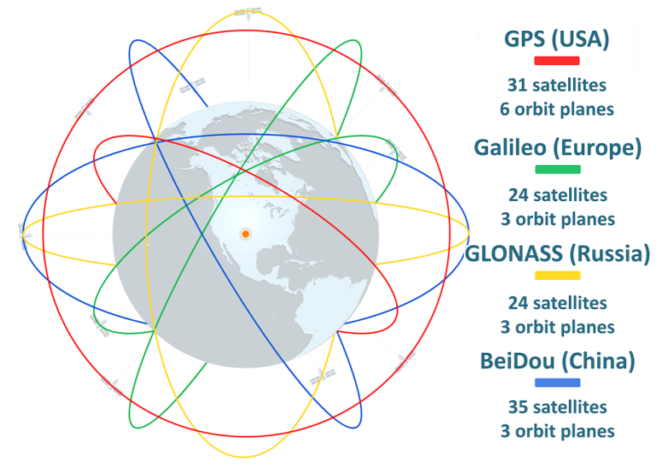
\includegraphics[width=\linewidth]{img/GNSS.png}}
                };
                \node[anchor=south east, inner sep=2pt] at (img.south east) { 
                    {{{\fontsize{3}{3.4}\selectfont\raggedleft \textcolor{black}{\textit{Credit:} \citeauthor{ramadan_HowDoesGNSS_} \cite{ramadan_HowDoesGNSS_}}}}}
                };
            \end{tikzpicture}
        \end{column}
    \end{columns}
\end{frame}

